
\documentclass[aps,pra,twocolumn,eqsecnum,showpacs]{revtex4}
\usepackage{bm, graphicx, amsmath}
\usepackage{bbm}
\usepackage[section]{placeins}
%\usepackage{bbm}
%\usepackage{epsfig}
\usepackage{amssymb,amsmath,amsthm}
\usepackage[mathscr]{eucal}


  %%%%%%%%%%%%%%%%%%%%%%%%%%%%%%%%%%%%%%%%%%%%%%%%%%%%%%%%%%%%%%%%%%%%%%% %%%%%%%%%%%%%%%%%%%%%%%%%%%%%%%%%%%%%%%%%%%%%%%%%%%%%
\newcommand{\id}{{\mathbb I}}
\newcommand{\tr}{{\rm tr}\,}
\newcommand{\ket}[1]{\left|{#1}\right\rangle}
\newcommand{\bra}[1]{\left\langle{#1}\right|}
\newcommand{\braket}[2]{\langle{#1}|{#2}\rangle}
\newcommand{\ketbrad}[1]{\left|{#1}\rangle\!\langle{#1}\right|}
\newcommand{\ketbra}[2]{\left|{#1}\rangle\!\langle{#2}\right|}
\newcommand{\mean}[1]{\langle{#1}\rangle}
\newcommand{\Qb}{\bar Q}
\parskip=1em
 


 \newcommand{\abs}[1]{\left|{#1}\right|}
 \newcommand{\av}[1]{\left\langle #1 \right\rangle}
 
  \newcommand{\br}[1]{\langle #1|}
  \newcommand{\ke}[1]{|#1\rangle}
  \newcommand{\bk}[2]{\langle #1|#2\rangle}
  \newcommand{\kb}[2]{\ke{#1}\br{#2}}
  \newcommand{\var}[2]{\langle #1,#2\rangle} 
  
  \newcommand{\al}[1]{^{(#1)}}
  \newcommand{\da}{^\dagger} 
  
  \newcommand{\pt}[1]{\left( #1 \right)}
  \newcommand{\pq}[1]{\left[ #1 \right]}
  \newcommand{\pg}[1]{\left\{ #1 \right\}} 
  
  \newcommand{\lpt}[1]{\left( #1 \right.}
  \newcommand{\lpq}[1]{\left[ #1 \right.]}
  \newcommand{\lpg}[1]{\left\{ #1 \right.}
  \newcommand{\rpt}[1]{\left. #1 \right)}
  \newcommand{\rpq}[1]{\left. #1 \right]}
  \newcommand{\rpg}[1]{\left. #1 \right\}} 
  
  \newcommand{\pp}[2]{ {\mbox{\scriptsize$
  \begin{array}{c}
  #1\\
  #2
  \end{array}$} } }  
  
  \begin{document}
  \title{Optimal discrimination of a class of mixed states with a fixed rate of inconclusive outcomes}
  \author{Vadim Yerokhin, Andi Shehu, and J\'{a}nos A. Bergou}

  \affiliation{Department of Physics and Astronomy, Hunter College of the City University of New York, 695 Park Avenue, New York, NY 10065, USA }
 
  
  \begin{abstract}
Recently the problem of optimal state discrimination with a Fixed Rate of Inconclusive Outcomes (FRIO strategy) has been solved for two pure quantum states and a few other highly symmetric cases. The strategy optimally interpolates between the Minimum Error discrimination strategy (fixed rate of inconclusive outcomes is zero) and the Unambiguous Discrimination strategy (fixed rate of inconclusive outcomes is the critical rate, $Q_{c}$, for which the error rate is zero). Here we extend the FRIO strategy to two mixed states, whose eigenvectors in their spectral representation form a Jordan basis. We derive the minimum error rate $P_{E}$ for a fixed inconclusive rate $Q$ and, in particular, the optimal distribution of the total $Q$ over the Jordan subspaces. As $Q$ is varied between the two limits, $0 < Q < Q_{c}$, a structure with multiple thresholds, $Q_{1}^{(th)} (=0) < Q_{2}^{(th)} < \ldots < Q_{N}^{(th)} < Q_{c}$, emerges. In the region, $Q_{1}^{(th)} < Q < Q_{2}^{(th)}$, one subspace receives the total $Q$. Above the second threshold $Q$ is shared by two subspaces, above the third threshold  by three, etc. Above the last threshold, $Q_{N}^{(th)} < Q < Q_{c}$, all subspaces participate in sharing $Q$.  The optimal measurement can be projective or a POVM and we give the conditions for the transition between the projective and POVM regimes.  The results are illustrated on the example of two rank 3 mixed states. 
 \end{abstract}
  \pacs{03.67.-a, 03.65.Ta,42.50.-p }
  \maketitle
  
  
%%%%%%%%%%%%%%%%%%%%%%%%%%%%%%%%%%%%%%%%%%%%%%%%%%%   INTRODUCTION   %%%%%%%%%%%%%%%%%%%%%%%%%%%%%%%%%%%%%%%%%%%%%%%%%%%%%%% %%%%%%%%%%%%%%%%%%%%%%%%%%%%%%%%%%%%%%%%%%%%%%%%%%%%%%%%%%%%%%%%%%%%%%%%%%%%%%%%%%%%%%%%%%%%%%%%%%%%%%%%%%%%%%%%%%%%%%%%%%%%%%%%%%
\section{Introduction}
\label{Intro}


In quantum information and quantum computing the information carriers are quantum systems and information is encoded in their state \cite{nielsen1}. Determining the state of the information carrier system is, therefore, a fundamental task in quantum information processing. Quantum state discrimination is one of the methods employed for this purpose and is the subject of this paper, while some of the others are, e.g., state estimation, tomography, and quantum learning.  

In state discrimination one deals with the following problem (for a recent review see \cite{bergourev}). One is given a quantum system that was prepared in one of $N$ known quantum states, $\{\rho_{i}|i=1,\ldots,N\}$, but we don't know which. The task is to identify the state, by performing some measurement on the system, as well as allowed by the laws of quantum mechanics. If the possible states are mutually orthogonal this is a relatively straightforward task: one just has to set up detectors along these orthogonal directions and determine which one clicks (assuming perfect detectors). However, if the states are not mutually orthogonal the problem is highly nontrivial and optimization with respect to some reasonable criteria leads to complex measurement strategies often involving generalized measurements (Positive Operator Valued Measures, POVMs).  Finding the optimum measurement strategy is the central task of state discrimination. 

The two fundamental state discrimination strategies are the so-called minimum-error (ME) strategy and the unambiguous discrimination (UD) strategy. In ME, every time a system is given and a measurement is performed on it a conclusion must be drawn about its state. Errors are permitted and in the optimal strategy the probability of making an error is minimized \cite{helstrom}. In UD, no errors are permitted at the expense of allowing an inconclusive measurement outcome to occur. When it occurs we don't learn anything about the state of the system and in the optimal strategy the probability of the inconclusive outcome is minimized \cite{ivanovic,dieks,peres,jaeger}. It has been recognized that states can be discriminated unambiguously only if they are linearly independent \cite{chefles1}. Discrimination with maximum confidence (MC) can be applied to states that are not necessarily independent and for linearly independent states it reduces to unambiguous discrimination \cite{croke,herzog1}, so it can be regarded as a generalized UD strategy. In the MC strategy Bayes' rule is used to maximize the chance of the appropriate detector clicking for its desired state.

It is clear that UD (or MC for linearly dependent states) and ME are the two extremes of a more general strategy and one can approach this more general strategy from either end. Starting from the UD end one can allow a fixed inconclusive rate $Q$ to occur that is smaller than the optimal (minimal) inconclusive rate $Q_{c}$ for UD, $0 \leq Q \leq Q_{c}$. Then one also needs to allow for errors to occur and one can minimize the error rate for the fixed value of $Q$. This scheme was introduced by Chefles and Barnett \cite{chefles2}, where they immediately provided the optimal solution for two pure states with equal prior probabilities, although at the time they did not prove full optimality of their solution. Later, Fiur\'{a}\v{s}ek and Je\v{z}ek \cite{fiurasek} generalized this result for mixed states. Useful bounds were obtained in Refs. \cite{zhang,eldar}, using the method of Semidefinite Programming (SDP). Alternatively,  one can start from the ME end and choose a certain fixed rate $P_{e}$ of errors to occur that is smaller than the optimal minimum error rate $P_{E}$, $0 \leq P_{e} \leq P_{E}$. Then one needs to allow for inconclusive outcomes to occur and one can minimize the inconclusive rate for a fixed value of $P_{e}$ \cite{touzel}. The first approach yields the minimal error rate as a function of the given inconclusive rate, $P_{e}(Q)$, while the second yields the minimum inconclusive rate as a function of the given error rate $Q(P_{e})$. Since the two expressions result from optimizations under different conditions, it is not immediately obvious that they are, in fact, the same (in the sense of being inverses of each other). It is relatively straightforward to prove, however, that this must be true and the proof is based on showing that the opposite leads to contradiction \cite{herzog2}. 

In a recent burst of activity both approaches were solved analytically for two pure states and for other, highly symmetric situations.   Actually, the second approach was solved earlier, first for two pure states with equal priors \cite{hayashi} and then for general occurrence probabilities \cite{sugimoto}. However the connection with the first approach remained unnoticed in these two works.  Quite recently, the first approach has been solved completely by two groups, using entirely different methods \cite{Bagan,Herzog1}.  Namely, Bagan  \textit{et al.} \cite{Bagan}
solved the problem introducing a transformation which formally eliminates the inconclusive part of the problem and reduces it to a ME problem with an extra optimization parameter. On the other hand, Herzog employed the SDP approach to obtain the solution for two pure states with arbitrary priors and for classes of special mixed states \cite{Herzog1}.

The goal of this paper is to extend the method developed in Ref. \cite{Bagan} to a class of mixed states whose spectral form is such that the eigenvectors form a Jordan basis for the Hilbert space of the problem. The UD of such mixed states has been investigated and the optimal solution has been obtained in \cite{HB,BFH}. Later this was extended to programmable quantum state discriminators, where in a different context the ME of such mixed states has been solved \cite{BBFHH}. Thus, we know both the UD and the ME limit for these states. In this paper we will derive the optimal strategy with a Fixed Rate of Inconclusive Outcomes (FRIO) that optimally interpolates between these two known limits. In particular, as the main finding of our paper, we will show that the optimal distribution of the fixed rate of inconclusive outcomes, $Q$, among the 2-dimensional subspaces spanned by the pair of Jordan basis vectors is highly non-trivial and an interesting threshold-like structure emerges: As we start increasing $Q$ from $Q=0$, first only one subspace receives the entire inconclusive rate. Then, as we increase $Q$ further, at a certain threshold a second subspace starts sharing the inconclusive rate. If we increase $Q$ further, at another threshold a third subspace also starts sharing $Q$, and so on, until above a last threshold all subspaces share the available  inconclusive rate. 


The paper is organized as follows. In Sec. \ref{sec:2} we briefly review the FRIO solution for two pure states, viz. the transformation solution found in \cite{Bagan}, because the treatment presented in the body of the paper relies heavily on this method. In Sec. \ref{sec:3} we extend the FRIO problem to 2 subspaces, each two-dimensional.  Then, in Sec. IV we consider a general Jordan Basis case, consisting of $N$ two-dimensional subspaces, where a Lagrangian optimization to minimize the error rate for fixed $Q$ over all subspaces leads to the threshold structure.  We illustrate the results on the example where the two mixed states to be discriminated are each of rank 3 and together they span a 6-dimensional Hilbert space. Because of the Jordan structure, the Hilbert space consists of three mutually orthogonal 2-dimensional Jordan subspaces.  In Sec. V we deal with the projective regimes separately. Finally, in Sec. VI we conclude with a discussion.  
%%%%%%%%%%%%%%%%%%%%%%%%%%%%%%%%%%%%%%%%%%%%%%%

\section{Review of the FRIO solution for two pure states}
\label{sec:2}

We first present a brief review of the method developed in \cite{Bagan} for the two pure state optimal FRIO problem since the rest of the paper relies heavily on this method.  We derive the maximum probability of success or, equivalently, the minimum probability of error in identifying the states, when a certain fixed rate of inconclusive outcomes is allowed. By varying the inconclusive rate, the scheme optimally interpolates between Unambiguous and Minimum Error discrimination (UD and ME), the two standard approaches to quantum state discrimination.

In all of these scenarios (UD, ME or FRIO) one is given a system which is promised to be prepared in one of two known pure states, $\rho_1= \ke {\psi_1} \br {\psi_1}$ or $\rho_2 = \ke {\psi_2} \br{\psi_2}$, but we don't know which. The pure states are prepared with prior probabilities $\eta_1$ and $\eta_2$, respectively, such that $\eta_1 +\eta_2 = 1$. It is well known that two pure states can be discriminated both unambiguously and with minimum error.  The optimal (minimal) inconclusive rate, $Q_{\rm c}$ for UD has been derived in \cite{ivanovic,dieks,peres,jaeger}, and is given by
\begin{equation}
    \label{Qmax}
    Q_{\rm c} = \left\{ \begin{array}{l}
     \eta_{1}+\eta_{2}\cos^{2}\theta, \mbox{if $\displaystyle \eta_{1} <
    \frac{\cos^{2}\theta}{1+\cos^{2}\theta}\equiv\eta_1^{(l)} $,}  \\ [.7em]
    \eta_{2}+\eta_{1}\cos^{2}\theta, \mbox{if $\eta_1>\displaystyle \frac{1}{1+\cos^{2}\theta}
    \equiv\eta_{1}^{(r)}$,}\\[.7em] 
   2\sqrt{\eta_{1}\eta_{2}}\cos\theta\equiv Q_0, \mbox{if $\eta_1^{(l)}\le\eta_1\le\eta_1^{(r)}$}\ ,
    \end{array}
    \right. 
\end{equation}
where $|\langle\psi_{1}|\psi_{2}\rangle| \equiv \cos \theta$ is the overlap of the states.

The optimal (minimal) error rate for ME has been derived in \cite{helstrom} and is given by
\begin{equation}
P_{\rm E}=\frac{1}{2}\left(1-\sqrt{1-4\eta_1\eta_2\cos^{2}\theta}\;\right).
\label{PE}
\end{equation}
For a compact derivation of these basic results see \cite{bergourev}.

In the FRIO strategy we want three measurement outcomes, one that we identify with the first state, one that we identify with the second state and one that we do not identify with a state, corresponding to the inconclusive outcome. Therefore, we look for the solution as a three-element POVM (Positive Operator Valued Measure),
\begin{equation}
\Pi_{1} + \Pi_{2} + \Pi_{0} = I \ ,
\label{POVM}
\end{equation}
where $I$ is the identity operator in the Hilbert space of the states. We identify a click in $\Pi_{1}$ ($\Pi_{2}$) with the first (second) state, while a click in $\Pi_{0}$ corresponds to the inconclusive outcome. We wish to optimize (maximize) the success rate, $P_s = \eta_1tr[\Pi_1 \rho_1] + \eta_2 tr[\Pi_2 \rho_2]$ or, equivalently, minimize the error rate, $P_e = \eta_1tr[\Pi_2 \rho_1] + \eta_2 tr[\Pi_1 \rho_2]$, for a fixed failure rate, 
\begin{equation}
Q = tr[\Pi_0(\eta_1 \rho_1 + \eta_2 \rho_2)] \ .
\label{Q}
\end{equation}
Obviously, $0 \leq Q \leq Q_{\rm c}$ and for $Q=Q_{\rm c}$ the FRIO strategy reduces to UD with $P_{e}=0$ while for $Q=0$ the FRIO strategy reduces to ME with the error rate given by \eqref{PE}. For a given intermediate value of $Q$ the strategy minimizes $P_e$.
 
The method of solution is based on the observation that, for optimal FRIO, $\Pi_{0}$ must be a rank one operator. Namely, if we assume the opposite, i.e., $\Pi_{0}$ is a rank two operator then it maps the two input states into a pair of other two states that can be further discriminated, contradicting that the strategy is optimal. The starting point is to write $\Pi_1+\Pi_2 = I - \Pi_0 \equiv \Omega$. Multiplying both sides of this equation by 
$\Omega^{-1/2}$  we have~$\tilde\Pi_1+\tilde\Pi_2 = I$,
where
\begin{equation}
\tilde\Pi_i=\Omega^{-1/2}\Pi_i \,\Omega^{-1/2}\ge0 .
\label{tildeops}
\end{equation}
So $\{\tilde\Pi_1,\tilde\Pi_2\}$ is a POVM.
Note that $\Omega^{-1/2}$ exists unless~$\Pi_0$ has a unit eigenvalue, in which case we address the problem differently (see later).
Defining the normalized transformed states $\tilde\rho_i$ and  \emph{a priori} probabilities $\tilde\eta_i$ as
\begin{equation}
\tilde\rho_i=\frac{\Omega^{1/2}\rho_i\Omega^{1/2}} {\tr(\Omega\rho_i)} ,  \qquad  \tilde\eta_i=\frac{\eta_i\tr(\Omega\rho_i)}{1-Q},
\label{tildestates}
\end{equation}
the error probability,~$P_{e}=(1-Q) \tilde P_{e}$, becomes 
\begin{eqnarray}
\tilde{P}_{e} &=& \tr(\tilde\eta_1\tilde\rho_1 \tilde\Pi_2)+\tr(\tilde\eta_2\tilde\rho_2 \tilde\Pi_1) ,
\label{tildePe}
\end{eqnarray}
and $\tilde{P}_{s} = 1 - \tilde{P}_{e}$. 
Equation \eqref{tildePe} and $\tilde\Pi_1+\tilde\Pi_2=\id$ define a ME discrimination problem for the transformed states and \emph{priors} given in Eq.~\eqref{tildestates}. The optimal solution to this ME discrimination problem immediately follows by using the tilde quantities in \eqref{PE}, with
$|\tilde\psi_i\rangle = \Omega^{1/2} |\psi_{i}\rangle /\sqrt{\langle\psi_{i}|\Omega|\psi_{i}\rangle}$ being the properly normalized transformed states.
  
Since the optimal~$\Pi_{0}$ is a positive rank one operator it can be written as $\Pi_0=\xi|0\rangle\langle0|$, where $\xi$ is its eigenvalue, $0\leq \xi \leq 1$, and the eigenstate belonging to $\xi$ is $|0\rangle$ and the orthogonal state is $|1\rangle$. In this basis $\Omega=(1-\xi)|0\rangle\langle0|+|1\rangle\langle1|$.
Writing the input states also in this basis, $|\psi_i\rangle=c_i|0\rangle+s_i|1\rangle$,
where $c_i\equiv\cos\theta_i$, $s_i\equiv\sin\theta_i$, and obtaining the transformed states and priors from Eq.~\eqref{tildestates}, after some simplifications we get
\begin{equation}
\tilde{P}^{\rm ME}_e=\frac{1}{2}\left\{1-\sqrt{1-4\eta_1\eta_2(\cos\theta-\xi c_1c_2)^2/(1-Q)^{2}} \right\} ,
\label{tildePe3}
\end{equation}
where we used that $\theta_{1} - \theta_{2} \equiv \theta$. It follows from~(\ref{Q}) that
%
\begin{equation}
\label{xi}
\xi=\frac{Q}{\eta_1c_1^2+\eta_2 c_2^2}.
\end{equation}
%
Hence Eq.~\eqref{tildePe3} depends only on one parameter, say~$\theta_1$, which determines the orientation of $\Pi_0$ relative
to that of the two pure states. The minimization over $\theta_1$ simplifies considerably, using Eq.~(\ref{xi}) and defining 
$ c_1\,\eta_1^{1/2}(\eta_1c_1^2+\eta_2c_2^2)^{-1/2}\equiv\cos\varphi$, and~$c_2\,\eta_2^{1/2}(\eta_1c_1^2+\eta_2c_2^2)^{-1/2}\equiv\sin\varphi$.
The resulting expression is minimum for~$\varphi=\pi/4$, yielding
%
\begin{equation}
P^{\rm min}_{e}\!=\!\frac{1}{2}\!\left\{1-Q - \sqrt{(1-Q)^2 - \left(Q_{0} - Q\right)^2}\right\} \ ,
\label{PeSol1}
\end{equation}
%
for all $Q \leq Q_{0}$, where $Q_0$ was introduced in the third line of~\eqref{Qmax}.
This is the optimal error rate for an intermediate range of the prior probabilities. 

For the validity of \eqref{PeSol1}, $\xi\le1$ must hold. 
The definitions of $\cos\varphi$ and $\sin\varphi$ after Eq.~(\ref{xi}) give
${\sqrt\eta_2 c_2=\sqrt\eta_1 c_1}$ for $\varphi=\pi/4$ which, in turn, leads to 
$\eta_1c_1^2=\eta_2c_2^2=\eta_1\eta_2\,{\sin^2\theta/( 1-Q_0)}$,
and~Eq.~\eqref{xi} yields $\xi=(1-Q_0)Q/(2\eta_1\eta_2\sin^2\theta)$.
Setting $\xi = 1$ defines the boundary $Q_{b}$, between the projective and POVM regimes, 
\begin{equation}
Q_{\rm b}\equiv {2\eta_1\eta_2\sin^2\theta/(1-Q_0)}.
\label{Qb}
\end{equation}
Hence~$\xi \leq 1$ if $Q \leq Q_{\rm b}$ and $\xi = 1$ if $Q > Q_{\rm b}$. 

In Fig. \ref{Fig1} we plot $Q_{\rm c}$ and~$Q_{\rm b}$ vs.~$\eta_{1}$ together for a fixed overlap, $\cos\theta = 0.5$ ($\theta = \pi/3$). The two curves intersect at $\eta_1=\eta_{1}^{(l)}$ and $\eta_1=\eta_{1}^{(r)}$, the same points as in Eq.~\eqref{Qmax}.
The interval $0 \leq \eta_{1} \leq 1$ is thus divided  into three regions. In regions~I and~III, we have $Q_{\rm b} < Q_{\rm c}$ and the solution~\eqref{PeSol1} is valid for $0 \leq Q < Q_{\rm b}$ only. In Region II, $\eta_{1}^{(l)} \leq \eta_{1} \leq \eta_{1}^{(r)}$, we have $Q_{\rm c} = Q_{0} < Q_{\rm b}$ and the solution \eqref{PeSol1} is valid for the entire $0 \leq Q \leq Q_{\rm c}$ range.

\begin{figure}[ht!]
    \centering{
      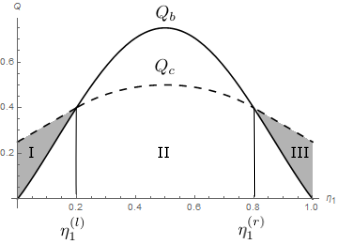
\includegraphics[height=4.5 cm]{Fig1.png}}
     \caption{$Q_{\rm c}$ (dashed line, Eq. \eqref{Qmax}) and $Q_{\rm b}$ (solid line, Eq. \eqref{Qb}) vs.~$\eta_{1}$ for $\theta=\pi/3$. Measurements can be optimized in the area under the dashed line, $Q_{c}$. Measurements in the area above $Q_{c}$ are suboptimal. In the shaded areas between $Q_{c}$ and $Q_{b}$ (regions I, left, and III, right) the optimal FRIO measurement is a projective measurement, in the unshaded area below $Q_{c}$ (region II) the optimal measurement is a POVM.}
     \label{Fig1}
     \end{figure}
 
In the shaded parts of regions I and III one has $Q_{\rm b} \leq Q \leq Q_{\rm c}$ and, necessarily, $\xi=1$. Hence,~$\Pi_0=|0\rangle\langle0|$ and $\Omega=|1\rangle\langle1|$ are projectors. Therefore,~$\Omega^{-1/2}$ does not exist in these areas and the case needs special consideration. 

The calculation of the error probability is most easily performed by realizing that $\Pi_1$ and $\Pi_2$ become degenerate, both must be
proportional to $\Pi_{d}=|1\rangle\langle1|$. The three-element POVM becomes a standard two element projective measurement,
$\{\Pi_d=|1\rangle\langle1|, \  \Pi_0=|0\rangle\langle0| \}$.
We identify a click in~$\Pi_{d}$ with $\rho_{1}$ ($\rho_{2}$)  if $\eta_1\ge\eta_2$ ($\eta_2\ge\eta_1$), so $P_{e(s)}=\eta_2 s_2^2, \quad P_{s(e)}=\eta_1 s_1^2$, with $Q=1-P_e-P_s$. These equations completely determine the solution. There is nothing to optimize here, so we drop the superscript $\rm min$ in what follows. $\theta_1-\theta_2=\theta$ immediately gives $Q(P_e)$ as
\begin{equation}
Q\!=\!1\! -\! P_{e}\! - \eta_{1(2)}\!\!\left(\!\sqrt{\!\frac{P_e}{\eta_{2(1)}}}\cos\theta\!\pm\!\sqrt{1\!-\!\frac{P_e}{\eta_{2(1)}}}\,\sin\theta\!\right)^{\!2}\!.
\label{PeSol2}
\end{equation}
Inverting this equation gives $P_e(Q)$ yields
\begin{widetext}
\begin{equation}
P_{e}=\eta_{2}\frac{2\eta_{1}\cos^{2}\theta(1-Q-Q_{2}) - (\eta_{1}-\eta_{2})(Q-Q_{2})-2\eta_{1}\eta_{2}\sin\theta\cos\theta\sqrt{Q(1-Q)-\eta_{1}\eta_{2}\sin^{2}\theta}}{1-4\eta_{1}\eta_{2}\sin^{2}\theta} \ ,
\label{PeSol2Exp}
\end{equation}
\end{widetext}
but the resulting expression is not particularly insightful.  However, we note that for $P_e=0$ (UD limit) one has~$Q=Q_{2}$, given by the second line in Eq.~(\ref{Qmax}), and for $Q = Q_{\rm b}$, $P_{e}$ reduces to \eqref{PeSol1}, as it should.



\section{Subspaces formalism: FRIO discrimination of two Rank 2 mixed states}
\label{sec:3}

In this and the next section we consider the FRIO discrimination of two mixed states that exhibit a Jordan structure. The two states, with their respective \emph{prior} probabilities $\eta_1$ and $\eta_2$,  are given in spectral (diagonal) form as, 
\begin{eqnarray}
 \rho_1 &=& \sum_{i=1}^{N} r_i \vert r_i \rangle \langle r_i \vert \nonumber \\
 \rho_2 &=& \sum_{i=1}^{N} s_i \vert s_i \rangle \langle s_i \vert \ . 
\label{rho1and2}
\end{eqnarray}
where $\langle r_{i}\vert r_{j}\rangle = \delta_{ij}$ and $\langle s_{i}\vert s_{j}\rangle = \delta_{ij}$. Each density matrix has rank $N$ and together they span a $2N$ dimensional Hilbert space. We assume that the Jordan condition,  
\begin{equation}
\langle r_i \vert s_j \rangle = \delta_{ij} \cos \theta_i \ ,
\label{jordan}
\end{equation}
holds so the set $\{\vert r_{i}\rangle, \vert s_{i}\rangle\vert i=1,\ldots,N\rangle\}$ forms a Jordan basis for the $2N$ dimensional Hilbert space. 

Due to the Jordan structure, instead of one $2N$ dimensional problem we have $N$ mutually orthogonal 2-dimensional subspaces. The $i^{th}$ subspace is spanned by $\vert r_i \rangle$ and  $\vert s_i \rangle$ with \emph{prior} probabilities $\eta_1 r_i$ and $\eta_2 s_i$, respectively.  The full discrimination of $\rho_{1}$ and $\rho_{2}$ can be accomplished by performing the discrimination in each subspace independently of the others, i.e., by discriminating $\vert r_i \rangle$ and  $\vert s_i \rangle$ in each subspace which is much simpler than the original problem. A physical implementation of this scheme is provided, e.g., by  the transmission of two input states over several optical fibers. Each fiber contains two degrees of freedom, that could be two orthogonal polarizations.

In the present section we will focus on the $N=2$ case when we have to deal with two 2-dimensional  subspaces only. We leave the general case of arbitrary $N$ to the next section.  
As discussed above, in this case we are dealing with two orthogonal 2-dimensional subspaces. 
The $i^{th}$ subspace is spanned by $\{\vert r_{i}\rangle,\vert s_{i}\rangle\}$ for $i=1,2$ and our task is to perform the optimal FRIO discrimination of  $\{\vert r_{i}\rangle$ and $\vert s_{i}\rangle\}$ within subspace $i$. The prior probability of $\vert r_{i}\rangle$ is $\eta_{1} r_{i}$ while the prior probability of $\vert s_{i}\rangle$ is $\eta_{2} s_{i}$. We define their normalized probabilities as 
\begin{eqnarray}
\eta_{1,i} &\equiv& \frac{\eta_{1} r_{i}}{\eta_{1} r_{i} + \eta_{2} s_{i}}, \nonumber \\ 
\eta_{2,i} &\equiv& \frac{\eta_{2} s_{i}}{\eta_{1} r_{i} + \eta_{2} s_{i}} \ ,
\label{etaij}
\end{eqnarray} 
such that $\eta_{1,i} + \eta_{2,i} = 1$.   

We now introduce a fixed rate of inconclusive outcomes for subspace $i$, $Q_{i}$,  such that $0 \leq Q_{i} \leq Q_{c,i}$ where $Q_{c,i}$ is given by Eq. \eqref{Qmax} with the obvious substitutions $\eta_{1} \rightarrow \eta_{1,i}$, $\eta_{2} \rightarrow \eta_{2,i}$ and $\cos \theta \rightarrow \cos \theta_{i} = \langle r_{i}\vert s_{i}\rangle$. We note that this reduces the problem to the FRIO discrimination of two pure states in subspace $i$, with prior probabilities given above. It follows immediately that the solution is given by \eqref{PeSol1} in the POVM regime of $Q_{i}$, $Q_{i} \leq Q_{c,i}, Q_{th,i}$, and \eqref{PeSol2} in the projective regime of $Q_{i}$, $Q_{th,i} < Q_{i} \leq Q_{c,i}$, again with the above substitutions.  

In the following we will focus mainly on the POVM regime where the solution in each subspace is given explicitly by Eq. \eqref{PeSol1},
\begin{equation}
P_{e,i} = \frac{1}{2} ( 1 - Q_i - \sqrt{ (1 - Q_i)^2 -(Q_{0,i} - Q_i )^2}) \ ,
\label{Pei2}
\end{equation}
where $Q_{0,i} = 2\sqrt{\eta_{1,i}\eta_{2,i}}\langle r_{i}|s_{i}\rangle$ ($i=1,2$). $Q_{0}$ was introduced in Eq. \eqref{Qmax} for the single subspace (two pure states) case, $Q_{0,i}$
 is its generalization for the case of two (or many) subspaces. We introduce the weight $\omega_{i}$ of subspace $i$ as 
\begin{equation} 
\eta_{1}r_{i} +\eta_{2}s_{i} = \omega_{i} \ ,
\label{omegai}
\end{equation} 
where, obviously, 
\begin{equation}
\omega_{1} + \omega_{2} = 1 \ .
\label{weights}
\end{equation} 
Then the total inconclusive rate is a weighted sum of the inconclusive rates of the individual subspaces, 
\begin{equation}
Q = \omega_{1} Q_{1} + \omega_{2} Q_{2} \ .
\label{Qtot2}
\end{equation}
We notice now that the total inconclusive rate $Q$ is fixed, with the fixed value satisfying $0 \leq Q \leq Q_{0}$, where
\begin{equation}
Q_{0} \equiv \omega_{1}Q_{0,1} + \omega_{2} Q_{0,2} \ , 
\label{Q0}
\end{equation}
is the maximal inconclusive rate that the two subspaces can accommodate.

Similary, the total error rate is a weighted sum of the error rates of the individual subspaces
\begin{equation}
P_{e} = \omega_{1} P_{e,1} + \omega_{2} P_{e,2} \ .
\label{Pe2}
\end{equation}
where $P_{e,i}$ is given in Eq. \eqref{Pei2}.


The task is to determine the optimal distribution of $Q$ between the two subspaces, the distribution that minimizes the total error rate $P_{e}$, under the constraint that $Q$ in Eq. \eqref{Qtot2} is fixed. 
Then only one of the $Q_{i}$s, say $Q_{1}$, is an independent variable, since $Q_{2} = (Q - \omega_{1} Q_{1})/\omega_{2}$. Inserting this into Eq. \eqref{Pe2} it becomes a function of the independent variable $Q_{1}$ and the optimization with respect to this variable is straightforward, yielding the optimal distribution of the fixed inconclusive outcomes between the two subspaces. 

In order to express the optimal failure rates in compact form it will be useful to introduce at this point the following convention. Without loss of generality in what follows we assume the hierarchy
\begin{equation}
Q_{0,1} \geq Q_{0,2} \ .
\label{hierarchy2}
\end{equation}
We also introduce the notation
\begin{equation}
Q_{th}^{(1)} \equiv 0 \ \ \ \ Q_{th}^{(2)} \equiv \frac{\omega_{1}(Q_{0,1} - Q_{0,2})}{1-Q_{0,2}} \ .
\label{Qth12}
\end{equation}
Then result of the optimization can be written as
\begin{eqnarray}
    \label{Q1opt}
    Q_{1}^{opt} = \left\{\begin{array}{ll}
    \frac{Q}{ \omega_{1} } & \mbox{if $Q_{th}^{(1)} \leq Q \leq   Q_{th}^{(2)}$}, \\
    \frac{1-Q_{0,1}}{1-Q_{0}}(Q - Q_{th}^{(2)}) + \frac{Q_{th}^{(2)}}{ \omega_{1} } & \mbox{if $ Q_{th}^{(2)} < Q \leq Q_{0}$},
    \end{array}
    \right. \nonumber \\
\end{eqnarray}
and
\begin{eqnarray}
    \label{Q2opt}
    Q_{2}^{opt} = \left\{\begin{array}{ll}
    0 & \mbox{if $0 \leq Q \leq  Q_{th}^{(2)} $}, \\
    \frac{1-Q_{0,2}}{1-Q_{0}} (Q-Q_{th}^{(2)})& \mbox{if $Q_{th}^{(2)} < Q \leq
    Q_{0} $} .
    \end{array}
    \right.
\end{eqnarray}
Clearly, Eq. \eqref{Qtot2} is satisfied by these solutions. 

A particular feature of the optimal solution is that it exhibits a threshold structure. The subspace with the larger $Q_{0,i}$, which is the first subspace following the hierarchy in Eq. \eqref{hierarchy2}, has the lower threshold. For $Q_{th}^{(1)}(=0) \leq Q < Q_{th}^{(2)}$ the second subspace does not accommodate any inconclusive outcome at all and it operates at the Minimum Error level. In this region of $Q$ all the inconclusive outcome is accommodated by the first subspace only. Above this threshold the two subspaces share the available inconclusive rate. If $\omega_{1}Q_{0,1} > \omega_{2}Q_{0,2}$, the first subspace always accommodates more inconclusive rate than the second, otherwise above some value of the total $Q$ the second subspace will accomodate more inconclusive rate than the first.  

The situation is depicted in Fig. \ref{Fig2}, for some specific values of the parameters.
\begin{figure}[ht,floatfix]
    \centering
$\begin{array}{c}
    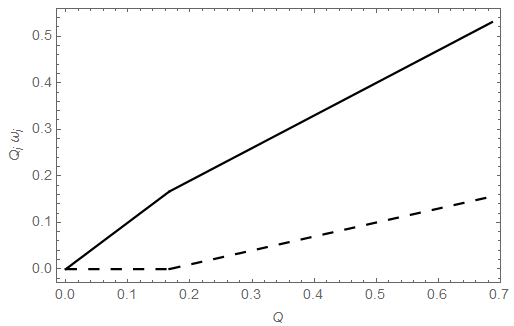
\includegraphics[height=4.5 cm]{Fig2a.png}  \\ 
\mbox{(a)} \\
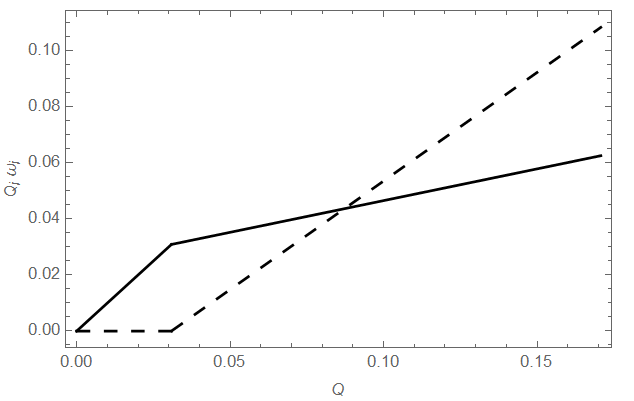
\includegraphics[height=4.5cm]{Fig2b.png} \\ \mbox{(b)} \\
\end{array}$
     \caption{$\omega_{1}Q_{\rm 1}^{\rm opt}$ vs. $Q$ (solid line) and $\omega_{2}Q_{\rm 2}^{\rm opt}$ vs.~$Q$ (dashed line). For the figure we used $\eta_{1}=\eta_{2}=1/2$ and the following parameter values: (a)  $\theta_{1}=\pi/4$, $\theta_{2}=2\pi/7$, $r_{1}=3/4$, $r_{2}=1/4$, $s_{1}=3/4$ and $s_{2}=1/4$; (b) $\cos\theta_{1}=1/4\sqrt{3}$, $\cos\theta_{2}=1/4$, $r_{1}=3/4$, $r_{2}=1/4$, $s_{1}=3/4$ and $s_{2}=1/4$.}
     \label{Fig2}
\end{figure}

Finally, inserting \eqref{Q1opt} and \eqref{Q2opt} into Eq. \eqref{Pei2} and using the resulting expressions in \eqref{Pe2} yields the optimal error probability, $P_{E}$, with a fixed rate of inconclusive outcomes,
\begin{widetext}
\begin{eqnarray}
    \label{PE2}
    P_{E} = \left\{ \begin{array}{ll}
     \frac{1}{2}\!\left\{1- Q - \sqrt{(\omega_{1} - Q)^2 - \left(\omega_{1}Q_{0,1} - Q\right)^2} - \sqrt{(\omega_{2} )^2 - \left(\omega_{2}Q_{0,2} \right)^2}\right\} & \mbox{ if $Q_{th}^{(1)} \leq Q \leq  Q_{th}^{(2)}$} \ , \\
    \frac{1}{2}\!\left\{1 - Q - \sqrt{(1-Q)^2 - \left(Q_{0} - Q\right)^2}\right\} & \mbox{ if $ Q_{th}^{(2)} < Q \leq
     Q_{0} $}  \ ,
    \end{array}
    \right.
\end{eqnarray}
\end{widetext}
which is the main result of this section. It is valid in all regions of the parameter $Q$. In particular, for the maximum allowable inconclusive rate, $Q=\omega_{1}Q_{0,1}+\omega_{2}Q_{2,0}$, Eq. \eqref{PE2} reduces to $P_{E}=0$, corresponding to optimal Unambiguous Discrimination of two subspaces \cite{HB,BFH}, while for $Q=0$ it reduces to the Minimum Error expression for two subspaces \cite{BBFHH}, as it should. We close this section by displaying $P_{e,i}$ vs. $Q$ in Fig. \ref{Fig3}, for some specific values of the parameters.

\begin{figure}[ht!]
\centering
$
\begin{array}{c}
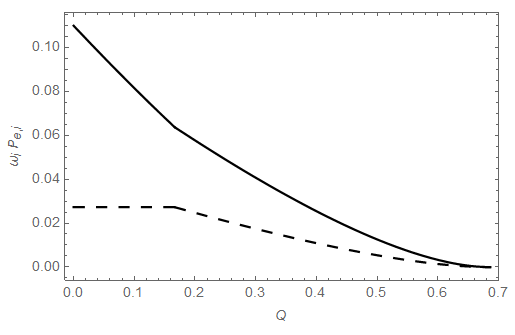
\includegraphics[height=4.5 cm]{Fig3a.png} \\
\mbox{(a)} \\
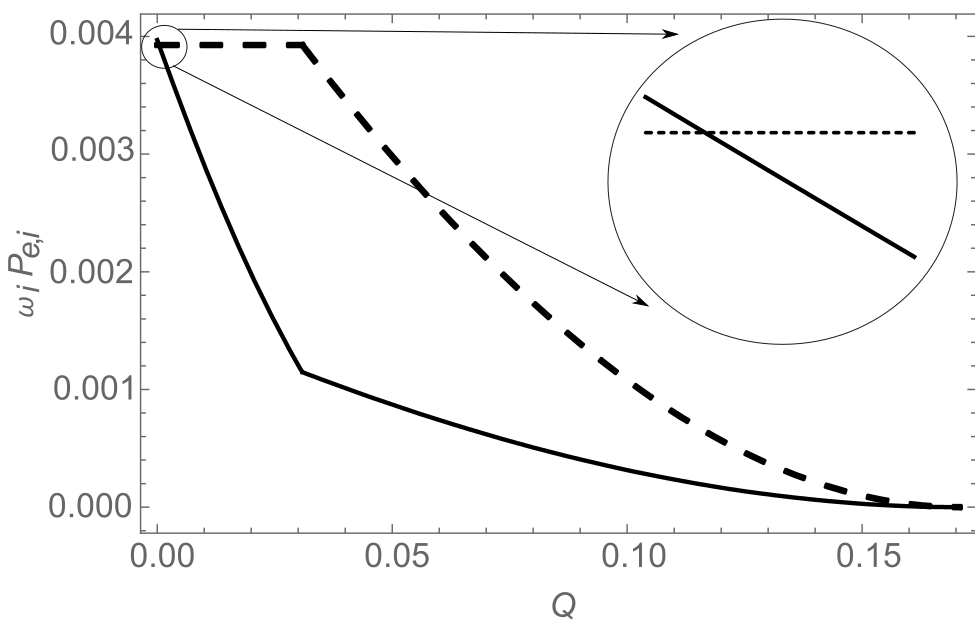
\includegraphics[height=4.5cm]{Fig3b.png} \\ \mbox{(b)} \\
\end{array}$
     \caption{$\omega_{1}P_{e,\rm 1}^{\rm opt}$ vs. $Q$ (solid line) and $\omega_{2}P_{e,\rm 2}^{\rm opt}$ vs.~$Q$ (dashed line). For the figure we used the same parameter values as in Fig. \ref{Fig2}. The insert in (b) shows that the solid and dashed lines intersect for a very small value of $Q$.}
     \label{Fig3}
     \end{figure}

\section{The general case: FRIO discrimination of two Rank $N$ mixed states, POVM regime}
\label{sec:4}

In this section we study the general case of two Rank $N$ density matrices, with $N$ being an arbitrary but fixed integer.  The two density matrices together span a $2N$ dimensional Hilbert space and their eigenvectors form a Jordan basis for the space. They are given in Eq. \eqref{rho1and2}.
The definitions and properties presented in Eqs. \eqref{jordan}--\eqref{omegai} remain  in effect but the part starting with Eq. \eqref{weights} has to be modified accordingly.
The weights of the subspaces, introduced in \eqref{omegai} now satisfy 
\begin{equation}
\sum_{i=1}^{N}\omega_{i} = 1 \ .
\label{Nweights}
\end{equation} 

The total inconclusive rate can again be written as a weighted sum of the inconclusive rates of the individual subspaces,
\begin{equation}
Q = \sum_{i=1}^{N}\omega_{i} Q_{i} \ .
\label{NQtot}
\end{equation}
$Q$ is fixed, with the fixed value satisfying $0 \leq Q \leq Q_{0}$, where now
\begin{equation}
Q_{0} \equiv \sum_{i=1}^{N}\omega_{i}Q_{0,i} \ , 
\label{NQ0}
\end{equation}
is the maximal inconclusive rate that the $N$ subspaces can accommodate.

Similarly, the total error rate is a weighted sum of the error rates of the individual subspaces,
\begin{equation}
P_{e} = \sum_{i=1}^{N}\omega_{i} P_{e,i} \ .
\label{NPe}
\end{equation}

The remaining task is to determine the optimal distribution of $Q$ between the $N$ subspaces, the distribution that minimizes the total error rate $P_{e}$, under the constraint that $Q$ in Eq. \eqref{NQtot} is fixed, i.e., to determine the optimal values of $Q_i$ as a function of the fixed $Q$. 

In order to perform the optimization we employ the Lagrange multiplier method because it leads to symmetric and easily tractable equations.  Adding $\lambda$ times the constraint, $Q -\sum_{i=1}^{N} Q_i = 0$, to \eqref{NPe} yields the constrained function
\begin{equation}
F = \sum_{i=1}^{N}\omega_{i}P_{e,i} + \lambda (Q - \sum_{i=1}^{N} \omega_{i}Q_i) \ ,
\label{constrainedF}
\end{equation}
where $P_{e,i}$ is inserted from Eq. \eqref{Pei2}, so it is also a function of $Q_{i}$. $\lambda$ is the Lagrange multiplier. 

Now, $Q_{i}$ and $\lambda$ can be treated as independent variables. Simultaneous optimization of $F$ with respect to $Q_{i}$ and $\lambda$ is straightforward. Before we present the results it will prove useful to introduce a hierarchy of the subspaces. So, in what follows we will assume 
\begin{equation}
Q_{0,1} \geq Q_{0,2} \geq \ldots \geq Q_{0,N} \ ,
\label{hierarchy}
\end{equation} 
which generalizes the ordering used in the case of two subspaces in the previous section. 

Then the optimal $Q_{i}$ can be written as
\begin{widetext}
\begin{eqnarray}
    \label{Qiopt}
    Q_{i}^{opt} = \left\{ \begin{array}{ll}
	\frac{1 - Q_{0,i}}{\sum_{i=1}^{k}\omega_{i} - \sum_{i=1}^{k}\omega_{i}Q_{0,i}}Q + \frac{Q_{0,i}\sum_{i=1}^{k}\omega_{i} - \sum_{i=1}^{k}\omega_iQ_{0,i}}{\sum_{i=1}^{k}\omega_{i} - \sum_{i=1}^{k}\omega_iQ_{0,i}} & \ \ \  \mbox{if $Q_{th}^{(k)} \leq Q \leq Q_{th}^{(k+1)}$ and $i \leq k$} \ , \\
0 & \ \ \  \mbox{if $i > k$} \ .
\end{array}
\right. 
\end{eqnarray}
\end{widetext}
Here $k=1,2,\ldots,N$ and we introduced the notation 
\begin{equation}
Q_{th}^{(k)} = \frac{\sum_{i=1}^{k}\omega_iQ_{0,i} - Q_{0,k}\sum_{i=1}^{k}\omega_{i}}{1 - Q_{0,k}} \ .
\end{equation}
and also $Q_{th}^{(N+1)} = Q_{0} = Q_{max}$, cf. \eqref{NQ0}. Obviously, for $k=1,2$ these results reproduce the results for two subspaces, Eqs. \eqref{Qth12}--\eqref{Q2opt}.

Inserting the optimal failure rates into the subspace-error rates $P_{e,i}$, \eqref{Pei2}, gives the optimal error rates for the subspaces, $P_{e,i}^{opt}$. Then using these optimal subspace-error rates in \eqref{NPe} 

gives the total optimal error rate $P_{E} = \sum_{i=1}^{N} P_{e,i}^{opt}$,

\begin{widetext}
\begin{eqnarray}
    \label{PEN}
    P_{E} = \left\{ \begin{array}{ll}
    \frac{1}{2}\left[1- Q - \sqrt{\left(\sum_{i=1}^{k}\omega_{i} - Q\right)^2 - \left(\sum_{i=1}^{k}\omega_{i}Q_{0,i} - Q\right)^2} - \sum_{i=k+1}^{N}\sqrt{(\omega_{i} )^2 - \left(\omega_{i}Q_{0,i} \right)^2}\right] & \mbox{ if $Q_{th}^{(k)} \leq Q \leq  Q_{th}^{(k+1)}$} \\
{} & \mbox{ and $k < N$} \ , \\
    \frac{1}{2}\!\left[1 - Q - \sqrt{(1-Q)^2 - \left(Q_{0} - Q\right)^2}\right] & \mbox{ if $ Q_{th}^{(N)} < Q \leq
     Q_{0} $}  \ ,
    \end{array}
    \right. 
\nonumber \\
\end{eqnarray}

\end{widetext}
which is valid in all regions of the parameter $Q$. For $N=2$, \eqref{PEN} reduces to the two-subspaces solution, \eqref{PE2}. For the maximum allowable inconclusive rate, $Q=Q_{0}$, the second line in Eq. \eqref{PEN} holds and it reduces to $P_{E}=0$, corresponding to optimal Unambiguous Discrimination of the subspaces \cite{HB,BFH}, while for $Q=0$ the first line holds and it reduces to the Minimum Error expression for $N$ subspaces \cite{BBFHH}, as expected. 




Again, the most interesting aspect of the optimal solution is that a structure with multiple thresholds emerges. For $Q_{th}^{(1)}=0 \leq Q < Q_{th}^{(2)}$ the total available inconclusive rate is accommodated by the first subspace only and all others operate at the Minimum Error level. According to the hierarchy introduced in Eq. \eqref{hierarchy}, the first subspace is the one with the largest $Q_{0,i}$. Then between $Q_{th}^{(2)} \leq Q < Q_{th}^{(3)}$ the second subspace, the one with the second largest $Q_{0,i}$ will also participate in sharing the available inconclusive rate, while the remaining $N-2$ subspaces continue to operate at the minimum error level.  In general, in the interval $Q_{th}^{(k)} \leq Q < Q_{th}^{(k+1)}$ the first $k$ subspaces share the available inconclusive rate and the remaining $N-k$ subspaces remain at the minimum arror level.  Finally, in the range $Q_{th}^{(N)} \leq Q \leq Q_{0}=Q_{max}$ all $N$ subspaces participate in sharing the available inconclusive rate. 

It is easy to show that the expressions are continuous at the threshold, i.e. the expressions valid below the threshold and the ones valid above the threshold tend to the same values at the threshold, although their slopes are, in general, different below and above the threshold. Furthermore, if $\omega_{i}Q_{0,i} > \omega_{i+1}Q_{0,i+1}$, the $i^{th}$ subspace always accommodates more inconclusive rate than the $i+1^{st}$ for all $i=1,2,\ldots,N$, otherwise above some value of the total $Q$ the $i+1^{st}$ subspace will accomodate more inconclusive rate than the $i^{th}$ subspace, the $Q_{i}^{opt}(Q)$ curves will intersect (see part (b) of Fig. \ref{Fig2} for an example).  

We illustrate these results on the example of $N=3$. In Fig. \ref{Fig4}, we plot the optimal failure rates $\omega_{i}Q_{i}^{\rm opt}$ and in Fig. \ref{Fig5}, we plot the optimal error rates $\omega_{i}P_{e,i}^{\rm opt}$ for the three subspaces as a function of the total failure rate $Q$ for some specific values of the parameters.
\begin{figure}[ht]
\centering
$%
\begin{array}{c}
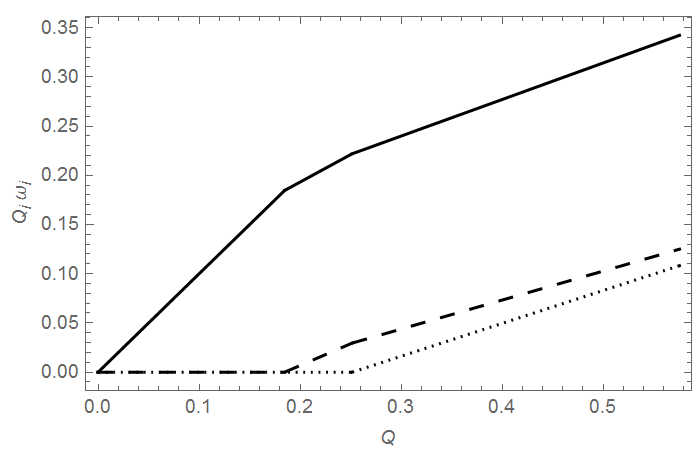
\includegraphics[height=4 cm]{Fig4.png} \\
\end{array}%
$%
\caption{Optimal subspace failure rates $\omega_{i}Q_{i}^{opt}$ vs. $Q$ from Eq. \eqref{Qiopt}, for three subspaces ($i=1,2,3$). $\omega_{1}Q_{1}^{opt}$: solid line. $\omega_{2}Q_{2}^{opt}$: dashed line. $\omega_{3}Q_{3}^{opt}$: dotted line. For the figure we used $\eta_{1}=\eta_{2}=1/2$ and the following parameter values: $\theta_{1}=\pi/4$, $\theta_{2}=\pi/3$, $\theta_{3}=\pi/3$, $r_{1}=5/8$, $r_{2}=1/4$, $r_{3}=1/8$, $s_{1}=3/8$, $s_{2}=1/4$ and $s_{3}=3/8$.}
\label{Fig4}
\end{figure}
\begin{figure}[ht]
\centering
$%
\begin{array}{c}
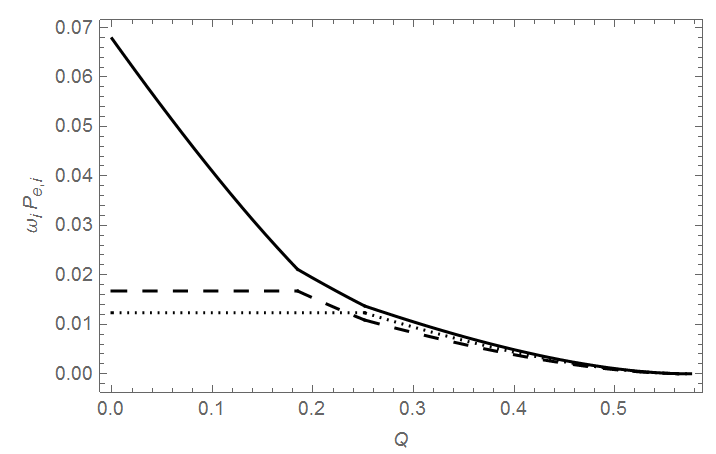
\includegraphics[height=4 cm]{Fig5.png} \\
\end{array}%
$%
\caption{Optimal subspace error rates $\omega_{i}P_{e,i}^{opt}$ vs. $Q$ from Eq. \eqref{Pei2} with \eqref{Qiopt}, for three subspaces ($i=1,2,3$). $\omega_{1}P_{e,1}^{opt}$: solid line. $\omega_{2}P_{e,2}^{opt}$: dashed line. $\omega_{3}P_{e,3}^{opt}$: dotted line. For the plots we used the same parameter values as for Fig. \ref{Fig4}.}
\label{Fig5}
\end{figure}

The results presented so far, in Sections III and IV, are valid if the parameters are such that in all subspaces we are in the POVM regime, i.e., $Q_{i}$ is in the unshaded region (region II) of Fig. 1 for all $i$. When the parameters are such that in some subspaces we are in the projective regime, i.e., $Q_{i}$ falls in the shaded regions of Fig. 1 (regions I and III) for some $i$ we have to modify the treatment to account for the fact that the error expression for the corresponding subspace, $P_{e,i}$, is no longer given by Eq. \eqref{Pei2} but by \eqref{PeSol2Exp}. We will study this case in the next section.  

\section{Projective regime}

We have seen in Section II for the single subspace case that the POVM solution is valid if the inconclusive rate is smaller than a boundary value, $Q \leq Q_{b}$, where $Q_{b}$ is given by Eq. \eqref{Qb}. With an obvious generalization, the POVM solution holds in subspace $i$ if in that subspace $Q_{i} \leq Q_{b,i}$ holds where the subspace boundary value is given by
\begin{equation}
Q_{\rm b,i} \equiv {2\eta_{1,i}\eta_{2,i} \sin^2\theta_{i}/(1-Q_{0,i})}.
\label{Qbi}
\end{equation}

In the region $Q_{b,i} \leq Q_{i} \leq Q_{c,i}$ the optimal measurement is a standard projective quantum measurement (SQM). The curves $Q_{b,i}$ and $Q_{c,i}$ intersect at $\eta_{1,i}=\eta_{1,i}^{(l)}$ and $\eta_{1,i}=\eta_{1,i}^{(r)}$, the same points as in Eq.~\eqref{Qmax}. The interval $0 \leq \eta_{1,i} \leq 1$ is thus divided  into three regions. In regions~I and~III, we have $Q_{\rm b,i} < Q_{\rm c,i}$ and the solution~\eqref{PeSol1} is valid for $0 \leq Q_{i} < Q_{\rm b}$ only. In Region II, $\eta_{1,i}^{(l)} \leq \eta_{1,i} \leq \eta_{1,i}^{(r)}$, we have $Q_{\rm c,i} = Q_{0,i} < Q_{\rm b,i}$ and the solution \eqref{PeSol1} is valid for the entire $0 \leq Q_{i} \leq Q_{\rm c,i}$ range.

Thus, Fig. \ref{Fig1} is valid in every subspace, with the obvious change of axis labels to $Q_{i}$ and $\eta_{1,i}$.  So, $Q_{i} > Q_{b,i}$ occurs in regions I and III and in the shaded areas the optimal FRIO measurement is an SQM while in the unshaded area it is a POVM. We now illustrate the case when the FRIO measurement is a POVM in one and an SQM in the other subspace on an example.  

The optimal distribution of the total available inconclusive rate $Q$ between the two subspaces, $Q_{1}^{opt}$ and $Q_{2}^{opt}$ such that their sum satisfies $Q_{1}^{opt} +Q_{2}^{opt}=Q$, can be found by optimizing the total error rate with respect to the failure rate of the subspaces. This is similar to the procedure followed in Sec. \ref{sec:3}, however we now have to use the error expression \eqref{PeSol2Exp} in subspace 1 for $Q>Q_{b,1}$. This leads to a numerical optimization problem, the result of which is shown in Fig. \ref{Fig6}.  


\begin{figure}[ht]
\centering
$%
\begin{array}{c}
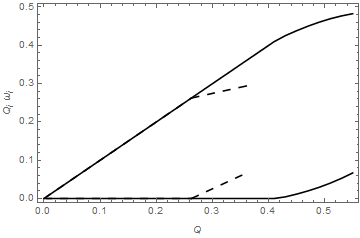
\includegraphics[height=4 cm]{Fig6.png} \\
\end{array}%
$%
\caption{Optimal subspace failure rates $\omega_{i}Q_{i}^{opt}$ vs. $Q$ from Eq. \eqref{Qiopt}, for two subspaces ($i=1,2,3$). $\omega_{1}Q_{1}^{opt}$: solid upper line. $\omega_{2}Q_{2}^{opt}$: solid lower line. The dashed lines indicate the behavior of the corresponding quantities if the POVM solution were valid for subspace 1.  For the figure we used $\eta_{1}=\eta_{2}=1/2$ and the following parameter values: $\theta_{1}=\pi/16$, $\theta_{2}=3\pi/7$, $r_{1}=9/10$, $r_{2}=1/10$, $s_{1}=1/10$ and $s_{2}=9/10$.}
\label{Fig6}
\end{figure}

The solution again exhibits a threshold structure. The dashed lines in the figure indicate how the optimal $Q_{i}$'s would behave if the POVM solution were valid for subspace 1 instead of the SQM. It is apparent that the SQM shifts the threshold toward a higher value of $Q$ and above the threshold the dependence on $Q$ is nonlinear, while for the POVM regime it is always linear.  

The optimal inconconclusive rate for subspace $i$, $Q_{i}^{opt}$, displayed in Fig \ref{Fig6}, is then inserted into Eq. \eqref{PeSol2Exp} for $i=1$ and \eqref{Pei2} for $i=2$. This yields the optimal error rate for subspace $i$, $P_{e,i}^{opt}$. The results are displayed in Fig. \ref{Fig7}. 

\begin{figure}[ht]
\centering
$%
\begin{array}{c}
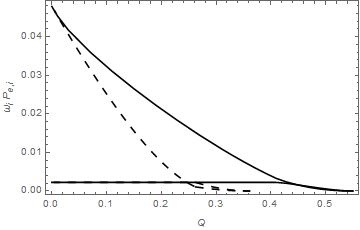
\includegraphics[height=4 cm]{Fig7.png} \\
\end{array}%
$%
\caption{Optimal subspace error rates $P_{e,i}^{opt}$ vs. $Q$ from Eq. \eqref{Qiopt}, for two subspaces ($i=1,2$). $P_{e,1}^{opt}$: solid upper line. $P_{e,2}^{opt}$: solid lower line. The dashed lines indicate the corresponding quantities if the POVM solution were valid in subspace 1. For the plots we used the same parameter values as for Fig. \ref{Fig6}.}
\label{Fig7}
\end{figure}
The optimal error rates also exhibit a threshold structure. Relative to the POVM regime, the SQM shifts the threshold to a higher value of $Q$ and the overall error rate also increases. 

\section{summary and conclusion} 
  
We have found analytic solutions for the optimal discrimination measurement strategy when a fixed rate of inconclusive outcomes, $Q$, is allowed (FRIO strategy), for a class of mixed states that exhibit a Jordan Basis structure.  Thus our work extends the previously introduced FRIO strategy from pure states \cite{Bagan} to  mixed states. In this strategy the probability of making an error in identifying the state, $P_{e}$, is minimized for a fixed $Q$ and the solution optimally interpolates between the minimum error ($Q=0$) and unambiguous discrimination ($P_{e}=0$) limits.  We found several surprising and unexpected conclusions.  The first is that the form of the optimal error rate remains formally the same over all subspaces as in the case of two pure states, which is a consequence of the Jordan structure of the mixed states. The second is a more striking feature, the emergence of a threshold structure: as we increase the allowed inconclusive rate $Q$, starting from $Q=0$, at first only one subspace accommodates all of the available $Q$. Above a certain threshold a second subspace starts sharing the available $Q$, above yet another higher threshold a third subspace starts participating, etc., until above a final threshold all of the subspaces participate. It is interesting to note that in this last regime the optimal error expression the second line in Eq. \eqref{PEN} is formally the same as the result for two pure states.  This is a novel type of  behavior and allows for experimental tests of our findings. Applications could be considered in cryptography where a key is shared over different lines to enhance security without sacrificing overall error rate. 

\begin{acknowledgments}
This publication was made possible through the support of a grant from the John Templeton Foundation. The opinions expressed in this publication are those of the authors and do not necessarily reflect the
views of the John Templeton Foundation. Partial financial support by a Grant from PSC-CUNY is also gratefully acknowledged. We also acknowledge useful discussions on various aspects of this project with Ed Feldman, Ulrike Herzog and Mark Hillery.
\end{acknowledgments}
  


  

\begin{thebibliography}{99}

     \bibitem{nielsen1}M. A. Nielsen and I. L. Chuang, \emph{Quantum Computation and Information} (Cambridge University Press, Cambridge, UK, 2000).
     \bibitem{bergourev}J.\ A.\ Bergou, Journal of Modern Optics \textbf{57}, 160 (2010).
     \bibitem{helstrom}C. W. Helstrom, \emph{Quantum Detection and Estimation Theory} (Academic Press, New York, 1976).
     \bibitem{ivanovic}I. D. Ivanovic, Phys. Lett. A \textbf{123}, 257 (1987).
     \bibitem{dieks}D. Dieks, Phys. Lett. A \textbf{126}, 303 (1988).
     \bibitem{peres}A. Peres, Phys. Lett. A \textbf{128}, 19 (1988).
     \bibitem{jaeger}G. Jaeger and A. Shimony, Phys. Lett. A \textbf{197}, 83 (1995).
     \bibitem{chefles1}A. Chefles, Phys. Lett. A \textbf{239}, 339 (1998).
     \bibitem{croke} S. Croke, E. Andersson, S. M. Barnett, C. R. Gilson, and J. Jeffers, \prl \textbf{96}, 070401 (2006).
     \bibitem{herzog1}U. Herzog, \pra \textbf{79}, 032323 (2009).
     \bibitem{chefles2}A. Chefles and S. M. Barnett, J. Mod. Opt. \textbf{45}, 1295 (1998).
     \bibitem{fiurasek}J. Fiur\'a\v{s}ek and M. Je\v{z}ek, \pra \textbf{67}, 012321 (2003).
     \bibitem{zhang}C.-W. Zhang, C.-F. Li, and G.-C. Guo, Phys. Lett. A \textbf{261}, 25 (1999).
     \bibitem{eldar}Y. C. Eldar, \pra \textbf{67}, 042309 (2003).
     \bibitem{touzel}M. A. P. Touzel, , R. B. A. Adamson, and A. M. Steinberg, \pra \textbf{76}, 062314 (2007).
     \bibitem{herzog2}U. Herzog, private communication around 2006; the proof is presented in \cite{Herzog1}.
     \bibitem{hayashi}A. Hayashi, T. Hashimoto, and M. Horibe, \pra \textbf{78}, 012333 (2008).
     \bibitem{sugimoto}H. Sugimoto, T. Hashimoto, M. Horibe, and A. Hayashi, \pra \textbf{80}, 052322 (2009).
     \bibitem{Bagan} E. Bagan, R Mu\~{n}oz-Tapia, G.A. Olivares-Renter\'{i}a and J.A. Bergou, \pra \textbf{86}, 040303(R) (2012).
     \bibitem{Herzog1}U. Herzog, \pra \textbf{86}, 032314 (2012).
     \bibitem{HB}U. Herzog and J. A. Bergou, \pra \textbf{71}, 050301R (2005).
     \bibitem{BFH}J. A. Bergou, E. Feldman, and M. Hillery, \pra \textbf{73}, 032107 (2006).
     \bibitem{BBFHH}J. A. Bergou, V. Bu\v{z}ek, E. Feldman, U. Herzog, and M. Hillery, \pra \textbf{73}, 062334 (2006).
     


\end{thebibliography}     
\end{document}
